\documentclass{report}
\usepackage[spanish]{babel}
\usepackage[utf8]{inputenc}
\usepackage{graphicx}
\usepackage{subfig}
\usepackage{amssymb, amsmath} %Paquetes matemáticos de la American Mathematical Society
\begin{document}
	%Portada
	\begin{titlepage}
		
		\begin{center}
			
\includegraphics[width=1cm, height=1.5cm]{ipn}
			\bfseries\LARGE Instituto Politécnico Nacional
			
\includegraphics[width=1cm, height=1.5cm]{escom}\par
			\bfseries\LARGE Instituto Politécnico Nacional \par
			\bfseries\LARGE Escuela Superior de Cómputo \par
			\vspace{3cm}
			\scshape\large PRACTICA 2: Complejidades temporales polinomiales y no polinomiales. \par
			\vspace{1cm}
			\large Tejeda Moyao Leon Francisco \par
			\itshape\large leontejeda@gmail.com \par
			\vspace{1cm}
		\end{center}
		
		
		\begin{bf}
			\large Resumen:
		\end{bf}
	
		\large En la presente practica se solicitó resolver 2 problemas, en los cuales se podría apreciar mejor el funcionamiento y la diferencia de rendimiento entre funciones recursivas y funciones iterativas.\par
			
		\bf\large Palabras Clave: Recursividad, Iteraciones, C, Fibonacci, \par
	\end{titlepage}
	\newpage
	
	\section*{Introducción.}
	\large  En esta practica se desarrollaron 2 problemas, el primero consistía en realizar un programa que encontrara el n-esimo número de la sucesión de Fibonacci de manera recursiva y de manera iterativa. Se debería de realizar el análisis apriori y aposteriori de la manera iterativa y el aposteori de la recursiva.\par
	\large  El segundo problema consistía en realizar 2 funciones, la primera función llamada Perfecto(N), la cual iba a indicar si un número era perfecto o no y realizar tanto el análisis a priori como el aposteori. Después de realizaría una función llamada MostrarPerfectos(N), la cual debería de mostrar los primeros N números perfectos y realizar su análisis aposteriori.\par
		
	\section*{Conceptos Básicos.}
	\large Para entender ciertos términos en esta práctica, se deberán de especificar a que se está haciendo referencia.\par
	\large Recurrencia, este termino hace referencia a la propiedad de aquellas secuencias en las que se puede calcular el siguiente termino sabiendo el valor de las que le preceden.\par
	\large Recursividad, este termino se utiliza en la programación, este hace referencia a que se pueden obtener conceptos nuevos empleando el mismo concepto que intenta describir.\par
	\large La serie de Fibonacci consiste en que la que para obtener un termino de esta, se deberán sumar las 2 posiciones anteriores.\par
	\begin{center}
		\large $n_0$=0 , $n_1$=1\par
	\end{center}
	\large Los números perfectos son los cuales al sumar todos sus divisores debe de dar el número al cual se está haciendo referencia.\par
	\newpage
	
	\section*{Experimentación y Resultados.}
	\begin{figure}[h]
		\large Para el primer problema se solicitaron 2 funciones, el algoritmo de Fibonacci de manera iterativa y de manera recursiva.\par
		\large Primero se realizó de manera iterativa y se realizaron los primeros 40 dígitos de la sucesión de Fibonacci. Se llegó a la conclusión de que no hay ni mejor ni peor caso, por el hecho de que siempre va tener que recorrer todo el arreglo.\par
		\large En la Figura 1: se puede observar los digitos y número de pasos obtenidos por el programa.\par
		\centering
			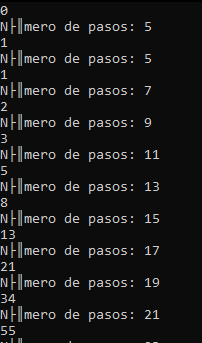
\includegraphics[width=4cm, height=6cm]{1} \par
		\caption{Fibonacci iterativo.}
	\end{figure}
	\newpage

	\begin{figure}
		\large Se procede a generar una gráfica en la herramienta DESMOS y es lo que se observa en la Figura 2.\par
		\centering
			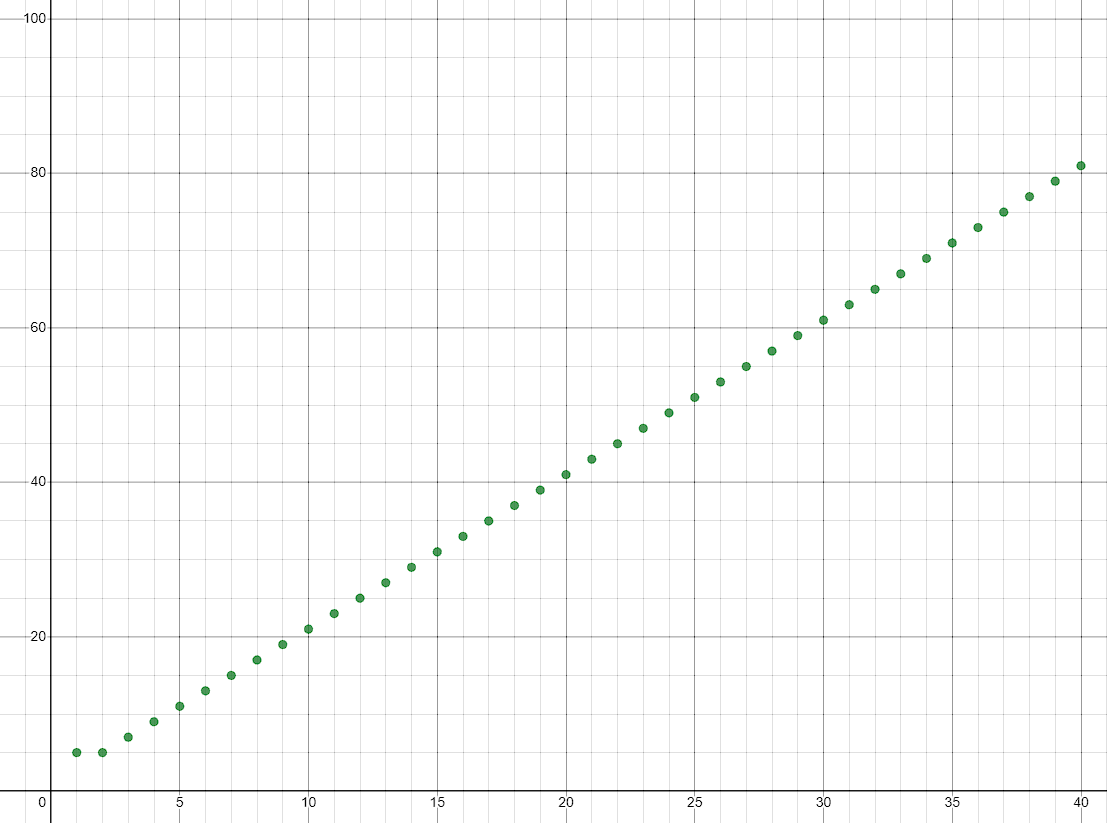
\includegraphics[width=10cm, height=5cm]{2} \par
		\caption{Grafica Fibonacci Iterativo.}
	\end{figure}
	
	\begin{figure}[h]
		\large En el analisis a priori (imagenes en el anexo), se llegó a la conlusión que T(N) $\epsilon$  $\theta$(N).\par 
		\large En la Figura 3 se puede observar como T(N) $\epsilon$  $\Omega$(N) ; T(N) $\epsilon$  O(N) \par
		\centering
			
\includegraphics[width=10cm, height=5cm]{3} \par
		\caption{Grafica funcion iterativa acotada.}
	\end{figure}
		
	\begin{figure}[h]
		\large En la Figura 4: se puede observar el comportamiento del código recursivo utilizando los 20 primeros números de fibonacci.\par
		\centering
			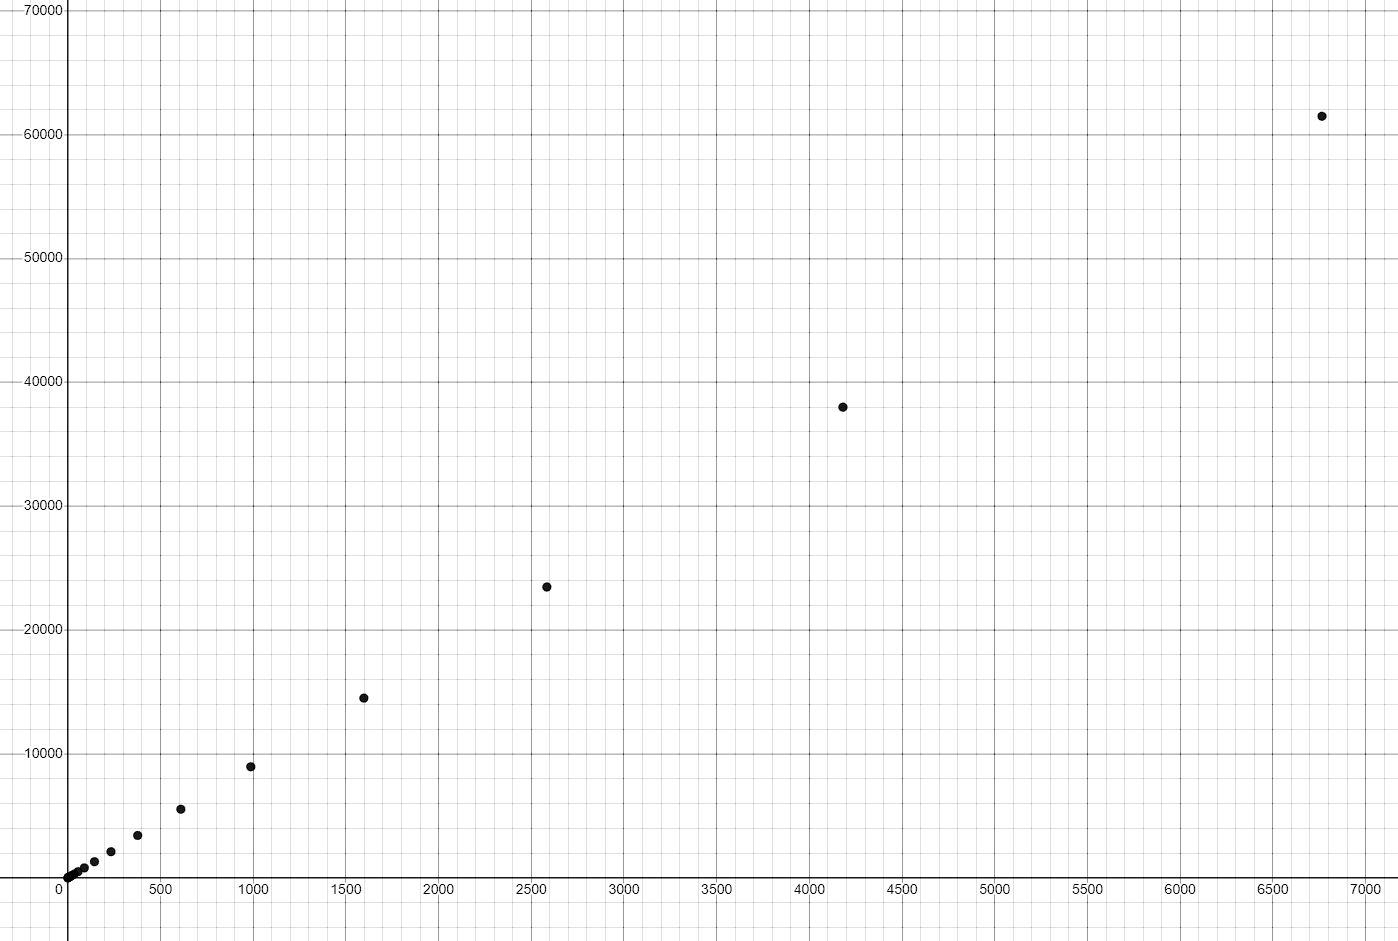
\includegraphics[width=10cm, height=5cm]{4} \par
		\caption{Grafica Fibonacci Recursivo.}
	\end{figure}
	\newpage
		
	\begin{figure}[h]
		\large Al igual que en la primera función, se puede observar que T(N) $\epsilon$  $\theta$(N).\par
		\large En la Figura 5 se puede observar como T(N) $\epsilon$  $\Omega$(N) ; T(N) $\epsilon$  O(15N) \par
		\centering
			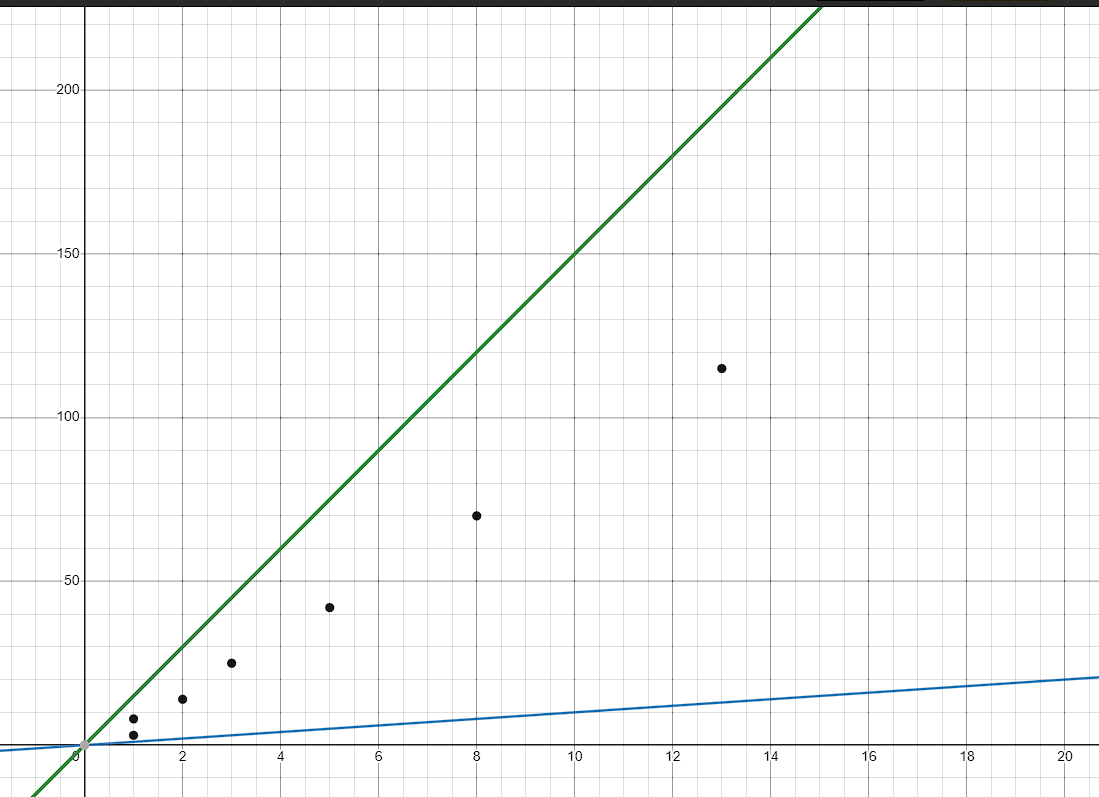
\includegraphics[width=10cm, height=5cm]{5} \par
		\caption{Grafica funcion recursiva acotada.}
	\end{figure}
	\newpage

	\section*{Conclusiones.}
	\begin{figure}[h]
		\begin{bf}
			\large Conclusiones Alumno 1: 
			
\includegraphics[width=1.5cm, height=1.5cm]{alumno} \par
		\end{bf}
		\large  En clase y viendo el comportamiento de los algoritmos, su llega a la conclusión de que hay ocasiones en donde convendrá usar funciones iterativas y otros escenarios en los cuales convendrá usar funciones recursivas.\par
		\large  Cada función cambia sobre a los recursos que utiliza. Las funciones iterativas ocupan tiempo y no ocupan demasiada memoria. Por otro lado, las funciones recursivas ocupan menos tiempo y mucha más memoria.\par
	\end{figure}
		
	\section*{Anexo.}
	\large Analisis apriori de la función iterativa de Fibonacci.\par 
	\begin{tabular}{| c | c | c |}
		\hline
		Fibo(int A[0, ..., n-1]. int n) & Costo & Número de pasos \\ \hline
		for(i=2; i<n; i++) & C1 & O(N-1)\\
		A[i] = A[i-1] + A[i-2] & C2 & O(1)\\ \hline
	\end{tabular}\par
	\large Se llega a la conclusión de que T(N) \O $\epsilon$  O(N).\par 
	
	\section*{Bibliografía.}
	\begin{itemize}
		\item \large Sucesión de Fibonacci: concepto, fórmulas y problemas resueltos. (s. f.). Recuperado 22 de octubre de 2022, de https://www.matesfacil.com/ESO/progresiones/sucesion-Fibonacci-formulas-problemas-resueltos-suma-espiral-triangulo-Pascal.html \par
		\item \large Recurrencia (s. f.). Recuperado 22 de octubre de 2022, de https://dle.rae.es/recurrencia\par 
		\item \large Recursividad: Conceptos básicos. (s. f.). Recuperado 22 de octubre de 2022, de https://www.tutorialesprogramacionya.com/javaya/detalleconcepto.php?codigo=123\par 
	\end{itemize}
\end{document}